\documentclass[a4paper,11pt]{memoir} 

\usepackage[utf8]{inputenc}
\usepackage[danish]{babel}
\usepackage[T1]{fontenc}
\usepackage[left=4.0cm, right=2.0cm, top=3.0cm, bottom=3.0cm]{geometry} 
\usepackage{amsmath,amssymb}																						

% SIUnitX  http://ctan.org/pkg/siunitx
\usepackage{siunitx,booktabs}		
\sisetup{per=slash}																						
\sisetup{per-mode = reciprocal}
\sisetup{inter-unit-product = \ensuremath{{}\cdot{}}}
\sisetup{output-decimal-marker = {,} }
\DeclareSIUnit{\kroner}{kr.}
\DeclareSIUnit{\LSb}{LSb}
\DeclareSIUnit{\cycles}{cycles}
\DeclareSIUnit{\div}{Div}

\usepackage{graphicx}
\newsubfloat{figure}% Allow subfloats in figure environment
\usepackage{dcolumn,booktabs}
\usepackage{url}
\usepackage{wrapfig}

% Redigere billed-/tabelteksterne.
\usepackage{caption}
\usepackage{subcaption}
\captionsetup{font=small,
	labelfont={it,bf},textfont=sf,
	format=hang}

% Packages for color handling
\usepackage[usenames,dvipsnames,svgnames,table]{xcolor}

\usepackage{threeparttable}

\usepackage{lscape}

\usepackage{enumitem}

% TODONotes http://ctan.org/pkg/todonotes
\usepackage{todonotes}
\usepackage{placeins}

\usepackage[hidelinks]{hyperref}  
\hypersetup{bookmarks=false}
\hypersetup{pdftitle={Batteristyresystem til Lithium Batterier}} 
\hypersetup{pdfsubject={7. semester afgangsprojekt}}
\hypersetup{pdfauthor={Kenneth Lukas Petersen, Søren Bolding Frank}}


% For includering af .pdf
\usepackage{pdfpages}

% Bibliografi
\usepackage{babelbib}
\bibliographystyle{abbrv}

% Noget forsideopsætning
\usepackage{soul} % lege lege
\sodef\an{}{0.2em}{.9em plus.6em}{1em plus.1em minus.1em}
\newcommand\stext[1]{\an{\scshape#1}}

% New commands 
\newcommand{\g}{9,82 \si{\meter\per\second\squared}}
\newcommand{\dcite}[1]{\quotedblbase{#1}\textquotedblright}
\newcommand{\husk}[2]{\todo[inline,color=green!40]{#1: #2}}
\newcommand{\jj}[1]{\todo[inline,color=green!40]{JJ: #1}}
\newcommand{\Kenneth}[1]{\todo[inline,color=blue!40]{Kenneth: #1}}
\newcommand{\note}[1]{\todo[inline]{#1}}
\DeclareMathOperator{\lapl}{\mathcal{L}}


% Remove paragraph indentation for document
\setlength{\parindent}{0pt}
\newcommand\hcancel[2][black]{\setbox0=\hbox{$#2$}%
	\rlap{\raisebox{.45\ht0}{\textcolor{#1}{\rule{\wd0}{1pt}}}}#2} 

% Listings package
\usepackage{listings}

%Fede overskrifter
\usepackage{kpfonts}
\usepackage{calc}
\setSingleSpace{1.0}
\SingleSpacing
\definecolor{chaptercolor}{gray}{0.8}
% helper macros
\newcommand\numlifter[1]{\raisebox{-2cm}[0pt][0pt]{\smash{#1}}}
\newcommand\numindent{\kern37pt}
\newlength\chaptertitleboxheight
\makechapterstyle{hansen}{
	\renewcommand\printchaptername{\raggedleft}
	\renewcommand\printchapternum{%
		\begingroup%
		\leavevmode%
		\chapnumfont%
		\strut%
		\numlifter{\thechapter}%
		\numindent%
		\endgroup%
	}
	\renewcommand*{\printchapternonum}{%
		\vphantom{\begingroup%
			\leavevmode%
			\chapnumfont%
			\numlifter{\vphantom{9}}%
			\numindent%
			\endgroup}
		\afterchapternum}
	\setlength\midchapskip{0pt}
	\setlength\beforechapskip{0.5\baselineskip}
	\setlength{\afterchapskip}{1\baselineskip}
	\renewcommand\chapnumfont{%
		\fontsize{3cm}{0cm}%
		\bfseries%
		\sffamily%
		\color{chaptercolor}%
	}
	\renewcommand\chaptitlefont{%
		\normalfont%
		%\huge%
		\LARGE%
		\bfseries%
		\raggedleft%
	}%
	\settototalheight\chaptertitleboxheight{%
		\parbox{\textwidth}{\chaptitlefont \strut bg\\bg\strut}}
	\renewcommand\printchaptertitle[1]{%
		\parbox[t][\chaptertitleboxheight][t]{\textwidth}{%
			%\microtypesetup{protrusion=false}% add this if you use microtype
			\chaptitlefont\strut ##1\strut}%
}}
\chapterstyle{hansen}
\aliaspagestyle{chapter}{empty} % just to save some space

%linje afstand
%\DisemulatePackage{setspace}
%\usepackage[nodisplayskipstretch]{setspace}
%\setstretch{0.5}
%\siglespacing
%\onehalfspacing                                       
%\doublespacing

%compile debug, check pdflatex time
\newcommand\showtimer{Timer: \the\numexpr\the\pdfelapsedtime*1000/65536 \relax}
%\pdfresettimer}
%\usepackage{fancyhdr}
%\pagestyle{fancy}
%\fancyfoot[CE,CO]{\showtimer}


\begin{document}
\begin{titlingpage}
\thispagestyle{empty}
\centering
{ \setlength{\baselineskip}{24pt}
{\Huge \stext{Digital grafisk equalizer til linjesignal} \par
%\textit{\&}\par
%\stext{Analogier}
}\par
\stext{Indlejrede systemer og signalbehandling - F17}
\par\vspace*{4\onelineskip}
\par
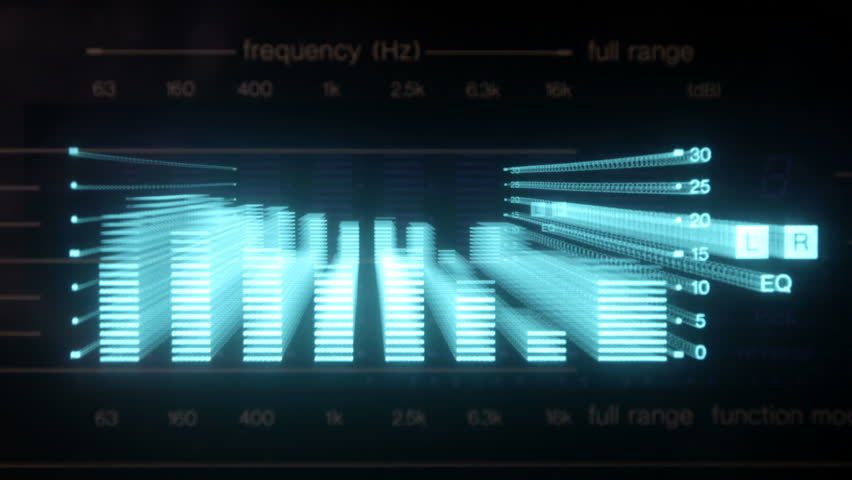
\includegraphics[width=10cm]{billeder/1.jpg}
\par\vspace*{4\onelineskip}
\stext{4. Semester Projekt}\par

\large\stext{J\"{o}rn Jacobi -- 230674}\par
\large\stext{Simon Juul M\o ller -- 230893}\par
\large\stext{S\o ren Frank -- 300595}\par
\large\stext{Dennis Amtoft Jensen -- ddmmyy}\par
\large\stext{Kenneth Petersen -- 161195}\par
\large\stext{Jonas Jensen Holmgren -- ddmmyy}\par

\vfill
\vspace*{2\onelineskip}
\stext{Gruppe 3}\par
\stext{Vejleder: Steffen Peter Skov }\par
\stext{1. februar - 26. maj 2017}\hfill
%\stext{24. maj 2013}\hfill
\par\vspace*{2\onelineskip}
\small
\stext{M\ae rsk Mc-Kinney M\o ller Instituttet}\par
\stext{Syddansk Universitet}
\enlargethispage{2\onelineskip}
}
\end{titlingpage}

\newpage

\renewcommand{\abstractnamefont}{\normalfont\bfseries}
\renewcommand{\abstracttextfont}{\normalfont}

\begin{abstract}
I dette projekt designes, realiseres og testes to forskellige versioner af et batteristyresystem. Den ene version realiseres ved hjælp af en dedikeret batteriovervågningskreds, og den anden uden denne kreds.
\\

Begge versioner realiseres ved hjælp af NXP LPC804 microcontroller serien. Batteristyresystemerne er designet ud fra samme kravspecifikation, men forskelle i ydeevne forekommer dog. En topologi for styresystemet blev valgt, hvorefter udviklingen af hardware og software til systemet blev påbegyndt.
\\

Systemet testes som en helhed og batteristyresystemernes funktionalitet og ydeevne eftervises.	
\end{abstract}

\thispagestyle{empty}

%---------- Indholdsfortegnelse  ---
\newpage
\thispagestyle{empty}
\null
\vfill
\begin{center}
\emph{Something something...}
\end{center}
\newpage
\thispagestyle{empty}
\null

\section*{Underskrifter}
\vspace{3ex} \hfill Underskrevet d. 24/05-2017\\

\newlength{\streg} \setlength{\streg}{0.49\linewidth}
\vspace*{\fill} \rule{\streg}{1pt} \hfill \rule{\streg}{1pt}\\
\begin{minipage}[b]{\streg}
 \centering
 \rule{0pt}{4ex}
 J\"{o}rn Jacobi \\
 {\footnotesize (230674) (jojac11@student.sdu.dk)}
\end{minipage}
\hfill
\begin{minipage}[b]{\streg}
 \centering
 Simon Møller \\
 {\footnotesize (230893) (simmo03@student.sdu.dk)}
\end{minipage}

\vspace*{\fill} \rule{\streg}{1pt} \hfill \rule{\streg}{1pt}\\
\begin{minipage}[b]{\streg}
 \centering
 \rule{0pt}{4ex}
 Søren Frank \\
 {\footnotesize (300595) (sofra15@student.sdu.dk)}
\end{minipage}
\hfill
\begin{minipage}[b]{\streg}
 \centering
 Dennis Amtoft Jensen \\
 {\footnotesize (ddmmyy) (dejen14@student.sdu.dk)}
\end{minipage}

\vspace*{\fill} \rule{\streg}{1pt} \hfill \rule{\streg}{1pt}\\
\begin{minipage}[b]{\streg}
	\centering
	\rule{0pt}{4ex}
	Kenneth Petersen \\
	{\footnotesize (161195) (kepet15@student.sdu.dk)}
\end{minipage}
\hfill
\begin{minipage}[b]{\streg}
	\centering
	Jonas Jensen Holmgren  \\
	{\footnotesize (ddmmyy) (jonho12@student.sdu.dk)}
\end{minipage}	
\newpage
\thispagestyle{empty}
\null
\vfill

\newpage
\thispagestyle{empty}
\chapter*{Forord}\label{chap:forord}
\addcontentsline{toc}{chapter}{Forord}

Udarbejdningen af dette afgangsprojekt er foretaget af studerende på 7. semester elektronik og datateknik, ved Syddansk Universitet, Teknisk Fakultet, efteråret 2018. Projektet er en sammenfatning af nogle af de opnåede fagligheder fra uddannelsens undervisning. Afleveringen af rapporten er dertil et krav for at kunne gå til eksamen.\\

Som udgangspunkt antages det at læseren har et tilsvarende fagligt niveau som en 7. semester studerende med linjefag indenfor elektronik og datateknik.
Rapporten tager derfor ikke hensyn til at skulle forklare den grundliggende viden, en studerende med samme faglige niveau antages at have.

\subsection{Læsevejledning}
Denne rapport er opbygget således, at den læses fra start til slut. Rapportens struktur er opdelt i hovedsektioner og undersektioner. Opbygningen er taksonomisk både i kapitelstrukturer og som helhed. Der vil i starten af hvert hovedafsnit være en figur som viser hvilken del af produktet der i det respektive afsnit bliver dækket.

\subsection{Arbejdsfordeling}
Arbejdsfordelingen har hovedsageligt været delt op i hardware og software. Kenneth har taget sig af hardwaren, mens Søren har udvilket softwaren til begge systemer. Der har gennem hele forløbet været tæt samarbejde, for at opnå en fuld forståelse af hele systemet for begge parter. 

\subsection{Typografiske konventioner}
Her er en kort oversigt over de typografiske konventioner der anvende i denne rapport\\
\begin{tabular}{l p{0.6\linewidth}}
	\textit{Kursiv tekst}			& Angiver filnavne i den tilhørende kodebase samt fremhævelse af ord eller fagudtryk. \\
	\textbf{Fed tekst}				& Bruges til a fremhæve produkt eller system specifikke betegnelser.\\
	\texttt{Konstant brede tekst}	& Anvendes til kildekode eksempler. Ligeledes anvendes afgrænsende områder.\\
	\emph{Fremhævet tekst}		    & Bliver brugt når der gives en kort introduktion til hvert kapitel.\\
\end{tabular}

\subsection{Typografi}
Rapporten har en opbygning, der gør den behagelig at læse og indeholder derfor mange tomme sider der er angivet med sidetal.
Det samlede antal reelle sider udgør 80 hele sider. 
\klp{Antal sider total}
\newpage
\thispagestyle{empty}
\null
\vfill

\newpage
\tableofcontents*												
\newpage

\SingleSpacing
%---------- Kalibrerings side --------
%Lorem ipsum dolor sit amet, pri ipsum partiendo interpretaris ea. Eum meliore persecuti no, at fugit quando mei. Nibh aliquid cum ei. Ne utinam libris nec, ex aliquip antiopam pri. Nam assum affert ancillae an, eos ea hinc mundi, dolor eleifend volutpat no usu. Ut nam esse essent ponderum. Ut eam quidam partiendo deterruisset, te pri consequuntur concludaturque. In oportere abhorreant vis, in usu ludus graeco volutpat, vel iudico dicunt prodesset ea. Mei natum noster eu, mei no ornatus ocurreret.
Pri unum maiestatis in, agam audiam perfecto ne mel. Ut per invenire petentium adolescens. An mei propriae phaedrum postulant. Vim amet electram ei. Ea wisi dolorem qui, mea propriae persecuti ad, option nusquam nominati ut mei. Nam te animal inermis, verear neglegentur ius id. His quem prompta inermis id, eruditi invidunt vix id. Eu sea tota vidisse deseruisse, aliquid nostrum voluptua ea vel. Facete audiam abhorreant an eum. Vim magna appellantur ne, vidit nulla sed ut. Mei nostrum vituperata consectetuer no. Noluisse placerat salutandi qui eu. Cum eu illud clita. Est vivendum convenire ex, sit primis iriure neglegentur an, ex sed modus tincidunt. Evertitur pertinacia constituam eu mea. Oblique alienum ocurreret ius ad. In eos aeterno iuvaret liberavisse, accusata euripidis an per. Nibh detracto placerat sea ut. Pri an minim aperiam omnesque, ancillae appareat reformidans ius in. Cibo aeterno erroribus ut eam, vim recteque scribentur liberavisse eu, choro soluta dolorem vis ea. Ad vel nullam graece legendos, sit melius menandri expetenda at. Sea inermis dolores ad, ut has noster argumentum. Qui movet zril an, in nam nobis quando. Usu ne saperet nostrum, per te nominati accusamus sententiae, est cu debet virtute accusata. Nihil fastidii his cu, pri aeterno persius vivendo id. Per te wisi temporibus, ullum iudicabit mea te, duis recusabo ea vel. Vim quodsi accumsan ut, te pro explicari iracundia. Vim id molestiae posidonium, clita everti facilisis ius te. Cu adhuc convenire comprehensam vis, decore facilis torquatos qui ne, at qui duis legendos sarium.
Zril commodo theophrastus cu cum. Eu reformidans conclusionemque sit, vix eu cibo everti similique, ex duo munere omnium principes. An vel sapientem moderatius, malis lobortis partiendo vel ne. Ea quod graeci expetenda usu.
Denne tekst er skrevet med Century Schoolbook fontstørrelse 11, med en afstand på 8pkt. efter afsnit og linjeafstand på 1.5.
%\newpage

%---------- Indledning -------------
\chapter{Indledning}

\emph{Lithium batterier er højtydende, langtidsholdbare og fås i forskellige former, hvilket gør dem velegnet til mange forskellige applikationer. De har dog ulempen at hvis de ikke overvåges kan de hurtigt forgå eller, i værste fald, kan der opstå farlige situationer. Derfor anvendes et batteristyresystem til opladning, afladning og vedligeholdelse. Batteristyresystemet overvåger konstant de individuelle celler og batteriet som helhed, for at sikre at parametrene er i orden. I denne rapport vil læseren blive guidet igennem processen bag udviklingen af et batteristyresystem.}

\section{Formål}
Formålet med dette afgangsprojekt er at udarbejde et produkt, der efterviser nogle af de opnåede fagligheder igennem uddannelsen som Diplomingeniør i Elektronik og Datateknik - både teoretisk og praktisk.

\section{Problemformulering}
Linak er gået ind på markedet indenfor reclinerstole, hvor et nyt aktuatorsystem er under udvikling. Da en batteripakke vil indgå i det samlede system, og den består af en seriekobling af lithium celler, er der brug for et batteristyresystem. Batteristyresystemet (BMS’en) vil sidde mellem batterierne og elektronikken for at styre op- og afladning af batteripakken, samt bidrage med sikkerhed i batteripakken. Problemformuleringen er derfor som følgende:\\

Et batteristyresystem ønskes udviklet og realiseret ved hjælp af en microcontroller og integrerede kredse eller transistorer. Det ønskes også at være muligt at se aktuel batteristatus via et display eller en konsol. Derudover ønskes det at batteristyresystemet kan overvåge 4-6 celler i serie. \\

Der ønskes også svar på følgende problemstillinger: 
\begin{itemize}[noitemsep]
	\item Hvordan opbygges en BMS ved hjælp af integrerede kredse?
	\item Hvordan opbygges en BMS ved hjælp af transistorer? 
	\item Hvordan fremstilles software til kontrol af batteripakken?
	\item Hvilken topologi af batteristyresystemer egner sig bedst til løsning af Linak's problemstilling? 
	\item Hvordan sikres der imod kortslutning og overcurrent/overvoltage? 
\end{itemize}

\section{Projektafgrænsning}
Under dette projekt designes et batteristyresystem, som skal kunne balancere en seriekobling af fire 18650 lithium celler. Der tilstræbes at designe og konstruere en funktionel prototype.
\subsection{Kravspecifikation} \label{afs:kravspecifikation}
Max aflade strøm (8A) \\
Balanceringsspænding (50mV opløsning) \\
Indgangsspænding fra oplader (18V)\\
"Låsning" af yderpunkter på batteriernes afladekurve (Brug af 80\%)



\begin{itemize}
	\item Opladning og afladning af Lithium celler
	\item Afladning under opladning
	\item Balancering under opladning og afladning v/ flere celler i serie
	\item Afladningsbeskyttelse/kortslutningsbeskyttelse
	\item Kontrol af maksimal lade- og afladestrøm
	\item Temperaturmålinger af celler for sikker drift
	\item State of charge
	\item State of health
\end{itemize}

\subsection{Vægtningsskema}

\section{Løsningsmodel}
Bliver udarbejdet senenere

\section{Læsevejledning}
Bliver udarbejdet senenere

\section{Proces- og arbejdsmetode}
Projektarbejdet er delt op i tre faser. Research og forberedelse, udvikling og test, færdiggørelse og konklusion. I research-fasen samles alt relevant information omkring emnet for at opnå en bedre forståelse. I udviklingsfasen fokuseres der på følgende punkter: 
\begin{itemize}
	\item Virkningsgrad
	\item Sikkerhed
	\item Modularitet
	\item Brugertilpasning
\end{itemize}


							

\listoftodos
%\newpage
\section{How To do stuff in LaTeX}

\subsection*{Figur, enkelt}
%-----------------------------------------------------------------------------
\begin{figure}[h!]
	\centering
		\includegraphics[width=.5\textwidth]{billeder/sample.png}
	\caption{Her skrives en god caption til figuren.}
	\label{fig:sample_fig_ref_her}
\end{figure}
\FloatBlock
%-----------------------------------------------------------------------------

\subsection*{Figur, dobbelt}
%-----------------------------------------------------------------------------
\begin{figure}
	\centering
	\subbottom[]{%
  		\includegraphics[width=.39\textwidth]{billeder/sample.png}
	  	\label{fig:sample_fig_ref_her_a}}
	\subbottom[]{%
		\includegraphics[width=.39\textwidth]{billeder/sample.png}
		\label{fig:sample_fig_ref_her_b}}
  	\caption{Her skrives en god caption til figuren.}
	\label{fig:sample_fig_ref_her_samlet}
\end{figure}
\FloatBlock
%-----------------------------------------------------------------------------

\subsection*{Kommentar}
%-----------------------------------------------------------------------------
\husk{Initialer}{Kommentaren skrives her}
%-----------------------------------------------------------------------------

\subsection*{Math Simple}
%-----------------------------------------------------------------------------
\begin{align}
D = \frac{1}{\Delta F}
\end{align}
%-----------------------------------------------------------------------------

\subsection*{Math uden nummer og align}
%-----------------------------------------------------------------------------
\begin{align}
D &= \frac{1}{\Delta F} \Rightarrow \nonumber \\
\Omega &= \mathrm{Noget helt andet}
\end{align}
%-----------------------------------------------------------------------------
\subsection*{Tabeller med caption}
\begin{table}
\centering
    \caption{Konstanter som bruges i overstående formler.}
\label{tab:konst1}
    \begin{tabular}{ | l | l |}
    \hline
    A & 18 [V] \\ \hline
    f & 50 [Hz]  \\ \hline
    T & 20 [s]  \\ \hline
    $\omega$ & 30 \\ \hline
    k & 100 \\ \hline
    \end{tabular}
    \end{table}

\newpage

%---------- Chapter ----------------
\chapter{Chapter}\label{kap:chap1}

%---------- Parts ----------------
\section{Section}\label{sec:sect1}

%---------- Chapter ----------------

%---------- Parts ----------------

%---------- Chapter ----------------

%---------- Parts ----------------

%---------- Chapter ----------------

%---------- Parts ----------------


%---------- Chapter ----------------
\chapter{Diskussion og vurdering}\label{kap:diskussion}
Valg af topologi blev modulær, da det var den ideelle løsning til antallet af celle i systemet. Da mange funktionaliteter skulle implementeres blev passiv balancering valgt, grundet dens simplicitet og effektivitet for balancering af cellerne.
\\

Strømmålingen blev realiseret i begge versioner med en $10\milli\ohm$ shunt modstand. I versionen med battery monitor kredsen anbefales en $1\milli\ohm$ shunt modstand, da den skal kunne måle en meget større strøm end nødvendig i dette projekt. 
\\

Der blev fundet fejl i schematics da PCB var bestilt. Oplde MOSFET'en blev koblet til detektering af afladestrøm og omvendt. Dertil blev der valgt forkert footprint til microcontrolleren på den diskrete version, hvilket skabte store problemer. 
\klp{Se om vi får det op at køre}							

%---------- Chapter ----------------
\chapter{Konklusion} \label{kap:konklusion}
Der kan igennem arbejdet med dette afgangsprojekt konkluderes at:							


\SingleSpacing

\nocite{*}
\bibliography{rapport}\label{bilag:litteratur}
%\listoffigures
%\listoftables

%--------- Bilag -------------------
\appendix
%\input{section/ord}
\chapter{Bilag}
%\input{section/symbol}
%\chapter{Stykliste} \label{bilag:styklister}
\begin{table}[h!]
	\small
	%\centering
	\label{tab:stykliste_ic}
	\begin{threeparttable}
		\begin{tabular}{p{0.25\linewidth}p{0.2\linewidth}p{0.25\linewidth}p{0.15\linewidth}p{0.05\linewidth}}
			%\begin{tabular}{ l l l l l l l }
			\toprule
			\multicolumn{1}{l}{\textbf{Komponent}}  &
			\multicolumn{1}{l}{\textbf{Værdi}}      &
			\multicolumn{1}{l}{\textbf{Type}}       &
			\multicolumn{1}{l}{\textbf{Bemærkning}} &  \\ 
			\hline
			C7                   & $\SI{1}{\nano\farad}$   & SMD 0603 &   \\
			C12, C13             & $\SI{2.2}{\nano\farad}$   & SMD 0603 &   \\
			C5, C10, C27         & $\SI{10}{\nano\farad}$  & SMD 0603 &   \\
			C3, C8, C9, C11, C16 & $\SI{100}{\nano\farad}$ & SMD 0603  &   \\
			C26                  & $\SI{100}{\nano\farad}$ & SMD 0805 &  $\SI{50}{\volt}$  \\
			C1, C2, C18, C19, C21, C22 & $\SI{1}{\micro\farad}$  & SMD 0603 &   \\
			C15, C24 & $\SI{1}{\micro\farad}$  & SMD 0805 &   \\
			C14 & $\SI{1}{\micro\farad}$  & SMD ELECTROLYT  & $\SI{50}{\volt}$  \\
			C20 & $\SI{4.7}{\micro\farad}$ & SMD 0603 &   \\
			C23, C25 & $\SI{10}{\micro\farad}$  & SMD ELECTROLYT  & $\SI{16}{\volt}$  \\
			C17 & $\SI{10}{\micro\farad}$  & SMD ELECTROLYT  & $\SI{35}{\volt}$  \\
			\midrule
			RS & $\SI{10}{\milli\ohm}$ & SMD 2512 &  $\SI{3}{\watt}$    \\
			R13, R14, R15, R28, R29, R30, R31& $\SI{22}{\ohm}$  & SMD 0603 &  $\SI{100}{\milli\watt}$ \\
			R19, R24, R25, R26, R32 & $\SI{100}{\ohm}$ & SMD 0603 & $\SI{100}{\milli\watt}$  \\
			R4, R5, R6, R7, R9 & $\SI{220}{\ohm}$ & SMD 0805 & $\SI{125}{\milli\watt}$ (a) \\
			R18, R20 & $\SI{1}{\kilo\ohm}$ & SMD 0603 & $\SI{100}{\milli\watt}$  \\
			R10 & $\SI{3.3}{\kilo\ohm}$ & SMD 0805 & $\SI{125}{\milli\watt}$  \\
			R8, R11, R112, R16, R21, R22, R23, R27, R33, R34 & $\SI{10}{\kilo\ohm}$ & SMD 0603 & $\SI{100}{\milli\watt}$  \\
			R17 & $\SI{22}{\kilo\ohm}$ & SMD 0603 & $\SI{100}{\milli\watt}$  \\
			R1, R2, R3 & $\SI{1}{\mega\ohm}$ & SMD 0603 & $\SI{100}{\milli\watt}$  \\
			R35 & $\SI{10}{\mega\ohm}$ & SMD 0805 & $\SI{125}{\milli\watt}$  \\
			\midrule
			Q1     & BSS84 & P-CH MOSFET &   \\
			Q3, Q4 & BC846B & BJT NPN &   \\
			Q5     & STL15DN4F5 & Dual N-ch MOSFET &   \\
			Q10    & 2N7002 & Logic level MOSFET &   \\
			\midrule
			S1, S3, S4 & SDTM-620-5mm  & TACT switch 5mm &   \\
			U1 & LM75BIM3 & $I^{2}C$ Temperatur måler &   \\
			U3 & BQ7692003PWR & BATTERY MONITOR &   \\
			MICROCONTROLLER & LPC804M101JDH22 & MICROCONTROLLER & \\
			U10 & TS9011SCX & $\SI{250}{\milli\volt}$ Low Quiescent &   \\
			Z10 & BZX84-C12 & $\SI{12}{\volt}$ zener diode&   \\
			D3, D4 & LED-G-3mm  & Grøn LED &   \\
			D5 & 1N5819 & Schottky diode &   \\
			PACK & CON-2X1-POLET & 2x1 polet stik - vinklet &   \\
			JP1, JP2 & HEADER03 & 3 pins - male &   \\
			UART, DISPLAY & HEADER04 & 4 pins - female &   \\
			CELL & HEADER05 & 5 pins - female &   \\
			\hline
			\bottomrule
		\end{tabular}
		\begin{tablenotes}
			\item[a] 2 stk $220\ohm$ 0805 i parallel som balanceringsmodstand.
		\end{tablenotes}
	\end{threeparttable}
	\caption{Stykliste for versionen med batteriovervågningskreds.}
\end{table} 


\begin{table}[h!]
\small
%\centering
\label{tab:stykliste_diskret}
\begin{threeparttable}
\begin{tabular}{p{0.25\linewidth}p{0.2\linewidth}p{0.25\linewidth}p{0.15\linewidth}p{0.05\linewidth}}
%\begin{tabular}{ l l l l l l l }
\toprule
\multicolumn{1}{l}{\textbf{Komponent}}  &
\multicolumn{1}{l}{\textbf{Værdi}}      &
\multicolumn{1}{l}{\textbf{Type}}       &
\multicolumn{1}{l}{\textbf{Bemærkning}} &  \\ 
\hline
C18, C19                  & $\SI{100}{\pico\farad}$ & SMD 0603       &   \\
C3                        & $\SI{1}{\nano\farad}$   & SMD 0603       &   \\
C2, C4, C7, C11           & $\SI{10}{\nano\farad}$  & SMD 0603       &   \\
C1, C5, C9, C10, C16, C17 & $\SI{100}{\nano\farad}$ & SMD 0603       & $\SI{50}{\volt}$  \\
C12, C14                  & $\SI{1}{\micro\farad}$  & SMD 0805       &   \\
C13, C15                          & $\SI{10}{\micro\farad}$ & SMD ELECTROLYT &   \\
\midrule
RS                                & $\SI{10}{\milli\ohm}$ & SMD 2512 &  $\SI{3}{\watt}$    \\
R6, R35                           & $\SI{10}{\ohm}$  & SMD 0603 & $\SI{100}{\milli\watt}$  \\
R64, R65, R66, R68, R69, R70, R71 & $\SI{22}{\ohm}$  & SMD 0603 &  $\SI{100}{\milli\watt}$ \\
R31, R32                          & $\SI{100}{\ohm}$ & SMD 0603 & $\SI{100}{\milli\watt}$  \\
R17, R21, R24, R27                & $\SI{150}{\ohm}$ & SMD 0805 & $\SI{125}{\milli\watt}$ (a) \\
R4, R30, R36, R37, R39, R41, R43  & $\SI{1}{\kilo\ohm}$ & SMD 0603 & $\SI{100}{\milli\watt}$  \\
R18, R20, R23, R26 & $\SI{3.3}{\kilo\ohm}$ & SMD 0805 & $\SI{125}{\milli\watt}$  \\
R1, R2, R5, R7, R8, R11, R13, R15, R33, R34, R67, R72, R73, R74 & $\SI{10}{\kilo\ohm}$ & SMD 0603 & $\SI{100}{\milli\watt}$  \\
R50, R51, R54, R55, R58, R59, R62, R63 & $\SI{15}{\kilo\ohm}$ & SMD 0603 & $\SI{100}{\milli\watt}$  \\
R28, R29, R49, R52, R53, R56, R57, R60, R61 & $\SI{22}{\kilo\ohm}$ & SMD 0603 & $\SI{100}{\milli\watt}$  \\
R47, R48 & $\SI{47}{\kilo\ohm}$ & SMD 0805 & $\SI{125}{\milli\watt}$  \\
R16, R19, R22, R25 & $\SI{100}{\kilo\ohm}$ & SMD 0603 & $\SI{100}{\milli\watt}$  \\
R45, R46 & $\SI{220}{\kilo\ohm}$ & SMD 0603 & $\SI{100}{\milli\watt}$  \\
R3, R14 & $\SI{270}{\kilo\ohm}$ & SMD 0603 & $\SI{100}{\milli\watt}$  \\
R12 & $\SI{330}{\kilo\ohm}$ & SMD 0603 & $\SI{100}{\milli\watt}$  \\
R9 & $\SI{470}{\kilo\ohm}$ & SMD 0603 & $\SI{100}{\milli\watt}$  \\
R10 & $\SI{10}{\mega\ohm}$ & SMD 0603 & $\SI{100}{\milli\watt}$  \\
\midrule

Q1, Q3, Q6, Q8, Q11, Q12, Q13, Q28 & BC846B & BJT NPN &   \\
Q2, Q4, Q5, Q7, Q9, Q27 & BC856B & BJT PNP &   \\
Q10 & 2N7002 & Logic level MOSFET &   \\
Q25 & STL15DN4F5 & Dual N-ch MOSFET &   \\

\midrule
D1, D2 & 1N5819 & Schottky diode &   \\
D3, D4 & LED-G-3mm  & Grøn LED &   \\
Z10 & BZX84-C12 & $\SI{12}{\volt}$ zener diode&   \\
S1, S2 & SDTM-620-5mm  & TACT switch 5mm &   \\
U1 & LPC804M101JHI33 & Microcontroller &   \\
U4, U5 & LM324-SMD-5GATES & Quad Op-Amp &   \\
U10 & TS9011SCX & $\SI{250}{\milli\volt}$ Low Quiescent &   \\
U12 & LM75BIM3 & $I^{2}C$ Temperatur måler &   \\
PACK & CON-2X1-POLET & 2x1 polet stik - vinklet &   \\
JP1, JP2 & HEADER03 & 3 pins - male &   \\
UART, DISPLAY & HEADER04 & 4 pins - female &   \\
CELL & HEADER05 & 5 pins - female &   \\

\hline
\bottomrule
\end{tabular}
\begin{tablenotes}
\item[a] 2 stk $150\ohm$ i parallel som balanceringsmodstand.
\end{tablenotes}
\end{threeparttable}
\caption{Stykliste for diskret version}
\end{table} 

%\input{section/tidsplan}
%\input{section/diagrammer}
%\input{section/cd_indhold}


\end{document}